% Fig. 1 of the paper — deployment workflow of the conformal temperature margin (layout spec: rounds/writing/fig1_spec.md).
% Build: pdflatex -output-directory=figs figs/fig_workflow.tex   (final width = one IEEE column, 88.9 mm; never rescaled)
\documentclass[border={1pt 1pt 3pt 1pt}]{standalone}
\usepackage{newtxtext,newtxmath}
\usepackage{tikz}
\DeclareMathSizes{7}{7}{7}{7}
\DeclareMathSizes{7.5}{7.5}{7}{7}
\DeclareMathSizes{8}{8}{7}{7}
\usetikzlibrary{positioning,fit,backgrounds,arrows.meta}
\definecolor{newfill}{HTML}{D6E6FA}
\definecolor{newline}{HTML}{1D5598}
\definecolor{grpfill}{HTML}{FFFFFF}
\definecolor{oldfill}{HTML}{F0F0F0}
\definecolor{oldline}{HTML}{6B7280}
\definecolor{ink}{HTML}{1F2937}
\newcommand{\hd}[1]{{\fontsize{8}{9.5}\selectfont\bfseries #1}}
\begin{document}
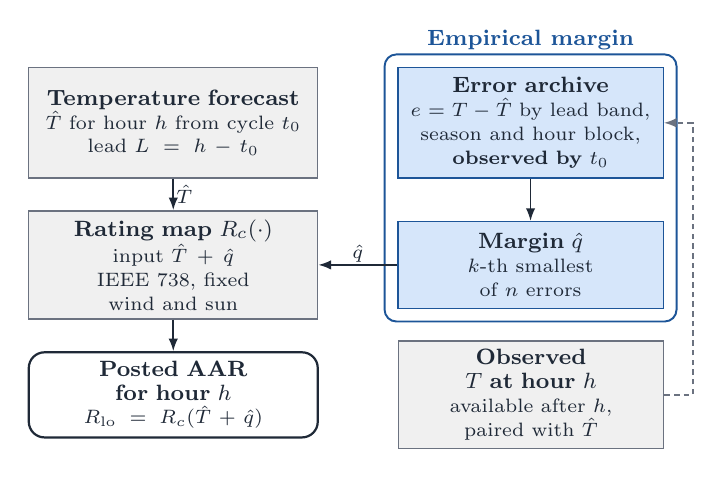
\begin{tikzpicture}[
    font=\fontsize{7.5}{8.6}\selectfont, text=ink,
    node distance=4mm and 10mm,
    box/.style={draw, line width=0.5pt, rectangle, align=center, minimum height=11mm, inner sep=1.1mm},
    oldL/.style={box, text width=34.5mm, fill=oldfill, draw=oldline},
    newR/.style={box, text width=31.5mm, fill=newfill, draw=newline},
    oldR/.style={box, text width=31.5mm, fill=oldfill, draw=oldline},
    post/.style={box, text width=34.5mm, fill=white, draw=ink, rounded corners=2mm, line width=0.8pt, minimum height=10mm},
    flow/.style={-{Latex[length=1.6mm]}, line width=0.6pt, draw=ink},
    later/.style={-{Latex[length=1.6mm]}, line width=0.6pt, draw=oldline, dash pattern=on 2pt off 1.5pt},
    lab/.style={font=\fontsize{7}{8}\selectfont, inner sep=0.8pt}
  ]
  \node[oldL, minimum height=14mm] (fc) {\hd{Temperature forecast}\\ $\hat T$ for hour $h$ from cycle $t_0$\\ lead $L = h - t_0$};
  \node[oldL, below=of fc] (map) {\hd{Rating map $R_c(\cdot)$}\\ input $\hat T + \hat q$\\ IEEE 738, fixed wind and sun};
  \node[post, below=of map] (aar) {\hd{Posted AAR for hour $h$}\\ $R_{\mathrm{lo}} = R_c(\hat T + \hat q)$};
  \node[newR, right=of fc, minimum height=14mm] (arch) {\hd{Error archive}\\ $e = T - \hat T$ by lead band,\\ season and hour block,\\ \textbf{observed by $\boldsymbol{t_0}$}};
  \node[newR, right=of map] (q) {\hd{Margin $\hat q$}\\ $k$-th smallest\\ of $n$ errors};
  \node[oldR, right=of aar] (obs) {\hd{Observed $T$ at hour $h$}\\ available after $h$,\\ paired with $\hat T$};
  \begin{scope}[on background layer]
    \node[draw=newline, fill=grpfill, line width=0.7pt, rounded corners=1.5mm, inner sep=1.6mm,
          fit=(arch) (q), label={[font=\fontsize{8}{9.5}\selectfont\bfseries, text=newline, inner sep=1pt]above:Empirical margin}] (grp) {};
  \end{scope}
  \draw[flow] (fc) -- node[lab, right] {$\hat T$} (map);
  \draw[flow] (arch) -- (q);
  \draw[flow] (q) -- node[lab, above] {$\hat q$} (map);
  \draw[flow] (map) -- (aar);
  \draw[later] (obs.east) -- ++(3.6mm,0) |- (arch.east);
\end{tikzpicture}
\end{document}
